\documentclass[preprint,authoryear]{elsarticle}
% \documentclass{article}
% \usepackage{graphicx}
\usepackage{amsmath}
\usepackage{amssymb}
\usepackage{amsthm}
\usepackage{multirow}
\usepackage{nicefrac}
\usepackage{graphicx}
\usepackage{subfig}

\newcommand{\taud}{\tau_d}
\newcommand{\taua}{\tau_a}
\newcommand{\ve}{\varepsilon}
\newcommand{\ltilde}{\tilde{l}}

\newtheorem{proposition}{Proposition}
\newtheorem{assumption}{Assumption}
\newtheorem{theorem}{Theorem}

\begin{document}

\title{Downtown tolls and the distribution of trip lengths }

\author[ll]{Lewis Lehe \corref{cor1}}

\address[ll]{UC Berkeley, Department of Civil and Environmental Engineering \\ lewis500@berkeley.edu \\ http://lewislehe.com}

\begin{abstract}

Currently, all downtown tolls are ``access tolls,'' meaning they charge for gross access to the zone, but tolls levied on distance-traveled are on the horizon. This paper shows how such tolls affect the distribution of trip lengths. A static model is presented in which travelers with potentially different trip lengths make a probabilistic choice of whether to enter a downtown zone governed by a Macroscopic Fundamental Diagram (MFD), with the choice probability declining as tolls and travel time rise. An application of Little's Law allows the model's equilibria to be derived in terms of a familiar supply/demand framework. Analysis proves and numerical simulation demonstrates that, if trip lengths and the value of a trip both vary across travelers, then access tolls inefficiently shift the distribution of car trip lengths toward long trips, whereas a distance toll can achieve the welfare-maximizing set of car trips.

\end{abstract}
\maketitle

\section{Introduction}

Economists usually recommend road tolls on the principle of marginal cost pricing---the idea that drivers should pay for their delay externalities. On a downtown network, what a rigorous application of this principle would mean is a web of differentiated tolls on every link \citep{Beckmann1956,YangHuang1998}. Obviously, such precision is impossible in practice. Instead,  Singapore \citep{Santos2004}, London \citep{santos2008,Leape2006}, Stockholm \citep{Eliasson2014}, Milan \citep{Gibson2015} and Gothenburg \citep{Borjesson2015} have all established downtown tolling systems that charge drivers, not on a link-by-link basis, but for the right to access a downtown zone. Hereafter, such systems will be classified as ``access tolls,'' because gross ``access'' to the downtown is what the driver buys from the toll authority. Meanwhile, Singapore has plans in place to switch to a satellite-based system that would charge drivers what will be called a ``distance toll,'' a charge per km travelled \citep{Tan2016}. Recently, Sadiq Khan, the Mayor of London, proposed replacing the current London Congestion Charge with some form of a distance toll \citep{Topham2017}.

This paper was inspired by an observation about how these systems are discussed: often the systems' initial design and later evaluation emphasizes changes in \emph{arrival} flows---the gross number of vehicles passing the tolled zone or crossing a cordon around it. As an example, the Stockholm Congestion Tax was designed with the goal of reducing traffic across the cordon by 10-15 percent \citep[p.396]{Eliasson2008}. As another, the designers of Singapore's Area License Scheme set the toll to reduce morning inbound traffic by 25-30 percent \citep[p. 12]{WatsonHolland1978}. 

The problem with this emphasis is that essential characteristics of traffic---its circulation, density and speed---depend, not only on the arrival flow's \emph{magnitude}, but also its \emph{distribution} by trip length. Consider a zone where half of all arriving vehicles park within a few blocks after crossing the boundary, while the other half are ridesharing vehicles that circulate endlessly. That zone could exhibit mild arrival flow alongside severe congestion, while a zone with higher arrival flow might have mild congestion if fewer ridesharing vehicles enter.

Of course, if enacting or raising a toll preserves the arrival flow's  distribution---that is, if it changes the number of trips of all lengths by the same proportion---then change in arrival flow might  be a fine proxy of how much the toll change has eased the burden on the street system. But what if toll changes \emph{do} change the trip length distribution? A little thought shows tolls might reasonably do so, since the rise in speed consequent to a toll change saves longer trips more time than short trips. Of course, with a distance toll, the inequality of travel time savings across trip lengths is attenuated by a money penalty on longer trips, but not with an access toll. To investigate such issues, this paper proposes and original static traffic model designed to show how downtown tolls might alter the trip length distribution and to uncover the consequences of that redistribution for social welfare and measurable traffic variables.

In designing such a model, a principal question is how best to represent traffic physics. One option is to have the downtown network be a graph of origins and destinations connected by links, which might have different capacities and wind up with different congestion levels. This is the approach taken by \citet{Meng2012}, \citet{Liu2013}, \citet{Verhoef2002b}, \citet{Lawphongpanich2012} and other studies in the ``second-best'' literature on feasible downtown tolls; this literature is devoted in large part to solution heuristics and algorithms, owing to the difficulty of finding optimal tolls and equilibrium route flows simultaneously. Similarly, \citet{May2000} experiments with different toll designs on a simulation of Cambridge. But while potentially useful for engineering real systems, the particularity of network modeling can bury insights that generalize across networks and populations.\footnote{Similarly, \citet{Mun2003} notes, ``Although network models are useful for practical applications, they are not suitable for investigating the general properties of the [pricing] problem, since the results depend on the network structures specified for calculations.''} In fact, for a network model it is not even exactly meaningful to speak of how something affects ``long trips'' or ``short trips,'' per se; if there is congestion on one side of the network but not the other, then two trips with the same length might have very different durations. Therefore, to avoid network modelling, we assume that traffic is spread sufficiently evenly across the network that a trip's duration depends only on its distance and on the network's space-averaged traffic conditions---not on the trip's origin, destination or route. Under this assumption, the network exhibits a stable relationship among space-averaged flow, density and speed called the Macroscopic Fundamental Diagram (MFD)\footnote{The relationship is also called the Network Fundamental Diagram (e.g., by \citet{Mahmassani2013}) or, splitting the difference, the Network Macroscopic Fundamental Diagram (e.g., by \citet{Laval2017}).}. Traffic readings have testified to the existence of MFD's in Yokohama \citep{Geroliminis2008} and Toulouse \citep{Buisson2009} among other places; and the MFD can even be derived analytically from network parameters in some cases \citep{Daganzo2008a,DaganzoLehe2016}.

The MFD approach is a popular one for studies of downtown tolling, and models in this vein---e.g., \citet{SmallChu2003}, \citet{Arnott2013}, \citet{Geroliminis2009a}---are sometimes called ``bathtub'' or ``isotropic'' models. What most distinguishes the model here from other isotropic models is (i) the static time character, (ii) variable trip lengths, and (iii) elastic demand arising from a random utility model. The static time character was chosen because dynamic models involve schedule preferences not essential to the topic (the question is \emph{whether} certain trips are driven, not \emph{when}) and require certain strong assumptions for tractability\footnote{See discussions of tractability in \citet{Fosgerau2015}, \citet{Daganzo2015}, \citet{Arnott2016} and \citet{Mariotte2017}.}. One similar study is \citet{Arnott2010}, which also features a static, isotropic model with elastic demand; if all trip were of the same length, then our model would be a special case of Arnott and Inci's in which parking is sufficient to preclude cruising. Another similar contribution is the elastic demand (Sec. 3) extension in \citet{Fosgerau2015}. In addition to the dynamic character of that model, a major difference here is that our travelers vary not only in their trip lengths but also in the benefit each derives from a car trip. This heterogeneous benefit makes the choice of a traveler with any given trip length probabilistic, so that the aggregate arrival flow of such trips rises smoothly with the trip's expected utility. As we shall see, this smoothly-changing demand draws out certain inefficiencies of an access toll that are supressed when either all $l$-length trips are driven or none are.

The paper is organized as follows: Section \ref{sec:model_setup} sets up the physics and demand mechanics of the model. Section \ref{sec:user_equilibrium} derives the untolled user equilibrium and shows how to frame the model in terms of both density congestion as well as flow congestion. Section \ref{sec:social_optimum} derives the model's social optimum. Sections \ref{sec:distance_tolls} and \ref{sec:access_tolls} show how to insert distance and access tolls, respectively, into the model and derives useful insights---the most important being that the distance toll can achieve the social optimum but the access toll cannot. Section \ref{sec:aggregates} shows how to calculate certain aggregates, to be used in Sec. \ref{sec:numerical_simulation}'s numerical simulations. Section \ref{sec:conclusion} concludes with ideas for further research and policy implications.

\section{Model setup}
\label{sec:model_setup}

This section describes the details of the paper's main model as composed of two sides: a ``physics'' side, describing how congestion occurs; and a ``demand'' side, describing how travelers choose whether to drive. The two sides are then linked by an application of Little's Law.

\subsection{Physics}
\label{ssec:physics}

The setting is a downtown zone governed by a Macroscopic Fundamental Diagram\footnote{For further background on the aggregate definitions involved in MFD modelling, see \citet{Daganzo2007}.}. A non-increasing function $v(k)$ (km/min) gives the space-averaged traffic speed $v$ (km/min) for a space-averaged density $k$ (veh/lane-km), but it will be convenient to use the inverse $p(k):=1/v(k)$ (min/km), which engineers call \emph{pace}. Minutes are the time-unit, rather than hours, to avoid having pace and circulation be small fractions in simulations. As Fig. \ref{fig:ue}a shows, $p(k)$ maintains a free-flow pace, $p_f$, for $k<k_f$, then rises monotonically.

Let $q$ (veh/min/lane) give the space-averaged ``circulation.'' By the traffic identity $q=kv$, there is a function
\begin{equation}
	q(k) := \frac{k}{p(k)}
\end{equation}
with the humped shape in Fig. \ref{fig:ue}b; it reaches a maximum $q_0$ at $k=k_0$ ($>k_f$). For densities $k<k_0$, blue highlighting denotes what is sometimes called ``light congestion,'' where $q$ rises as $k$ and $p$ rise. In light congestion, the addition of cars to the road may diminish speed, but not by so much as to lower the circulation. For $k>k_0$, traffic is ``hypercongested,'' meaning $q$ falls as $p$ and $k$ rise. In hypercongestion, the addition of cars lowers pace enough that circulation falls.

\begin{figure}
	\centering
	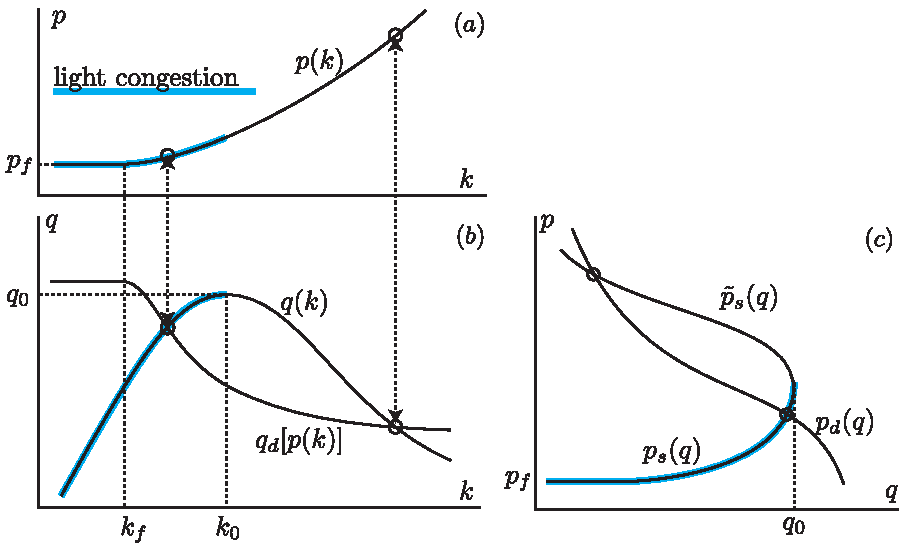
\includegraphics[width=1\textwidth]{img/equilibrium-k}
	\caption{User equilibria along the MFD.}
	\label{fig:ue}
\end{figure}

\subsection{Demand}
\label{ssec:demand}

There is a continuum of ``travelers'' who might potentially drive every minute. A traveler $i$ is characterized by a tuple $(\ve_i,l_i)$, where $l_i$ (km) is $i$'s trip length and $\ve_i$ (min) is $i$'s ``gross benefit'' from a car trip, measured in minutes of travel time. The utility of a car trip to traveler $i$, when there are no tolls and the pace of traffic is $p$, is
\begin{equation}
	U_i := \ve_i - pl_i.
\end{equation}

A traveler who chooses not to drive earns utility 0. We will call the choice not to drive the ``outside option,'' which could ostensibly represent traveling by another mode, choosing a route that does not pass through the downtown, or cancelling the trip. Note that this specification of utility is restrictive in at least two ways: (i) utility is perfectly linear in travel time, and (ii) the value of travel time does not vary across the population. 

The population is distributed with joint density $f(\ve,l)$. The densities of $l$ and $\ve$ are potentially independent, but, arguably, the two properties are likely to be positively correlated: travelers with long trips might be engaged in ridesharing, deliveries or trips to the airport, or they might not have good transit alternatives. The total mass of travelers is $\lambda$ (veh/min/lane-km), so that 
$$
\lambda \int_{l=l_0}^{l=l_1}\int_{\ve=\ve_0}^{\ve=\ve_1}f(\ve,l)d\ve dl
$$
gives the mass of travelers with gross benefits in $[\ve_0,\ve_1]$ and trip lengths in $[l_0,l_1]$. This integral, like all integrals hereafter, is written with the variable of integration in the limits, for clarity.

Before passing to the derivations, we will clarify two points about interpretation. First, the trip length is limited to \emph{intrazonal} travel only; any travel accomplished en route to the zone or after exiting the zone is outside the scope of the model. Second, due to the static time character, the ``population'' of travelers cannot be  thought of as a single, fixed crowd of people; rather, travelers stand in for a flow of constantly-generated trip opportunities, so the ``population'' is constantly refreshed with a continuum of travelers from an identical distribution.

\subsection{Little's Law}

``Little's Law'' is a classic result from queueing theory that states ``under steady state conditions, the average number of items in a queuing system equals the average rate at which items arrive multiplied by the average time that an item spends in the system'' \citep[p. 82]{Little2008}. The relationship turns out to be useful in linking arrival flows---as determined by demand---to traffic conditions.

Let $L$ be the lane-km of the network (the network being equivalent to the ``queueing system'' of Little's Law), $k^l$ the traffic density of travelers with $l$-length trips, and $a^l$ the rate at which such travelers arrive per lane-km. It follows that the number of such travelers on the road at once is $Lk^l$, and the rate at which they arrive in the whole network is $La^l$. The time such a traveler spends in the network, during a steady state with speed $v$, is $l/v$, so Little's Law can be stated
\begin{equation}\label{eq:little}
	Lk^l = (La^l) \left( \frac{l}{v}\right).
\end{equation}
Multiplying by $v/L$ yields
\begin{equation}
	q^l = a^l l,
\end{equation}
where $q^l$ is the circulation of travelers with $l$-length trips (derived from $q^l=k^lv$). Thus, given knowledge of arriving traffic in the steady state, we can learn the total circulation---even without measuring speed or density directly---by calculating and summing the circulations that correspond to each trip length.

\section{User equilibrium (UE)}
\label{sec:user_equilibrium}

\subsection{Derivation}
\label{ssec:derivation}

We now derive the UE that prevails without tolls. Since the outside option grants utility $0$, $i$ drives if and only if
\begin{equation} \label{eq:v-epsilon}
 \ve_i \geq pl_i.
\end{equation}

Figure \ref{fig:density} shows the resulting division of travelers between drivers and not-drivers, with shading that denotes the population density in the $l$-$\ve$ plane. The line $D(l): = lp$ divides traffic, such that every traveler above $D$ drives and none below does.
\begin{figure}
	\centering
	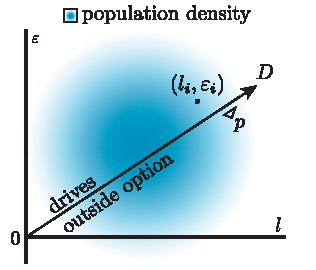
\includegraphics[width=0.55\textwidth]{img/mode-split3}
	\caption{distribution of population in untolled UE}
	\label{fig:density}
\end{figure}

If every traveler satisfying (\ref{eq:v-epsilon}) does drive, then, by Little's Law, circulation will be
\begin{equation}\label{eq:q_d}
		q_d(p) := \lambda \int_{l=0}^{l=\infty} \int_{\ve=lp}^{\ve=\infty} l f(\ve,l) d\ve \, dl \,\, \textnormal{(veh/lane/min).}
\end{equation}
This is the ``circulation demanded'' and is equal to the total mass above $D$ in the figure, weighted by the $l$'s. Note that even though the demand of an individual traveler---from the perspective of a toll authority who cannot measure $\varepsilon_i$---is probabilistic, the \emph{aggregate} circulation demanded, $q_d$, is deterministic. Also, distinguish $q_d$ from the \emph{arrival} flow demanded:
\begin{equation}\label{eq:a_d}
	a_d(p) := \lambda \int_{l=0}^{l=\infty} \int_{\ve=lp}^{\ve=\infty} f(\ve,l)d\ve dl \,\, \textnormal{(veh/lane-km/min)},
\end{equation}
which is not weighted by trip lengths.

A UE occurs when the choices expressed in $(\ref{eq:q_d})$ coincide with the physics that give rise to them---i.e., when $k=k^e$ such that
\begin{equation}\label{eq:equilibrium-n}
	q_d[p(k^e)] = q(k^e).
\end{equation}
The two sides of this equation appear in Fig. \ref{fig:ue}(b), where their intersections are UE. Note that there do not have to be exactly two user equilibria nor that one occur in light congestion.

So far we have proceeded in terms of $k$, $p$ and $q$ together, but a more traditional way to frame a static traffic model is in terms of $p$ and $q$ alone---as in Fig. \ref{fig:ue}(c). This framing, often called ``flow congestion'' technology, comes from \citet{Walters1961} and invites graphical comparisons to microeconomic concepts such as marginal cost. Let $p_s(q)$ map $q(k)\rightarrow p(k)$ on $[0,k_0]$ (light congestion), let $\tilde{p}_s(q)$ do so on $(k_0,\infty]$ (hypercongestion), and let $p_d(q):=q_d^{-1}$ give the pace inducing $q$. Figure \ref{fig:ue}(c) shows $p_s(q)$, $\tilde{p}_s(q)$ and $p_d(q)$. The first two curves, taken together, form a ``supply'' or ``average cost'' curve, while the $p_d(q)$ is the inverse demand curve. Intersections are, as before, the model's user equilibria. 

\subsection{Choice of equilibria}
\label{ssec:choice_of_equilibria}

A question naturally arises as to which equilibria matter, since $q_d(p)$ and $q(k)$ might intersect many times. To answer, we make two assumptions.
\begin{assumption}\label{ass:light-congestion}
If a lightly-congested equilibrium exists, then it will happen.
\end{assumption}
This assumption makes the most sense if one thinks of the equilibrium as having been reached by the zone filling up from a near-empty state. The lightly-congestion equilibrium would be the first equilibrium reached as $k$ rises, and so traffic might reasonably be expected to stay there.

On the other hand, suppose demand is so high that there are only hypercongested equilibria. There are two types of hypercongested equilibria possible, shown in Fig. \ref{fig:hypercongestion}. Those like $E_1$, where $q_d[p(k)]$ cuts $q(k)$ from above (i.e., where $q_d[p(k)]$ is steeper than $q(k)$), will be called \emph{Type 1}; those like $E_2$, where the opposite holds, will be called \emph{Type 2}. There is much discussion in the literature as to which type satisfies various stability criteria for static models of traffic on highways; see summaries in \citet{Verhoef1999}, \citet{Verhoef2005} and \citet{SmallChu2003}. Our own physics builds on the following assumption:

\begin{figure}
	\centering
	\subfloat[1][]{
	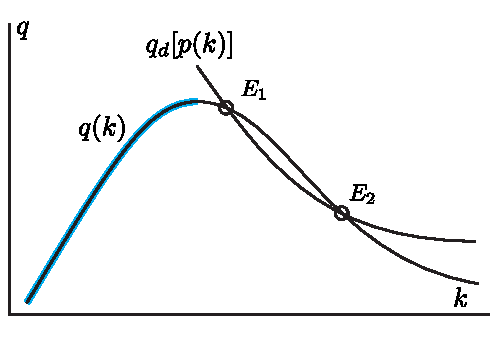
\includegraphics[width=0.52\textwidth]{img/hypercongestion}
	}
	\subfloat[2][]{
	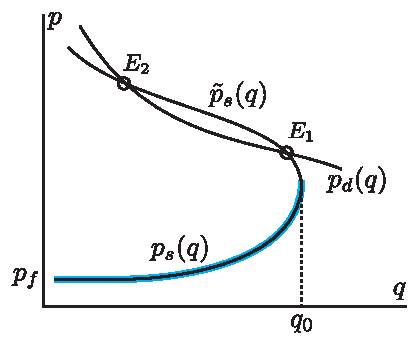
\includegraphics[width=0.5\textwidth]{img/hypercongestion-flow}
	}
	\caption{Types of hypercongested equilibria.}
	\label{fig:hypercongestion}
\end{figure}

\begin{assumption}\label{ass:type1}
If a lightly-congested user equilibrium does not exist, the network achieves the Type 1 equilibrium with the lowest density/highest circulation.
\end{assumption}

This assumption is justified by the analysis in \citet{Arnott2010}, which shows that Type 1 equilibria satisfy all the stability criteria that the authors consider for a static isotropic model with elastic demand, whereas Type 2 equilibria are stable only in a restricted sense. Their arguments are deep, but the following mental exercise can make the point intuitive. Reasonably, $q_d$ is a quantity related to instantaneous arrival flow; it tells the circulation one would expect to measure if the magnitude and composition of arrival flow induced by a pace $p$ were sustained. Meanwhile, $q(k)$  measures instantaneous vehicle motion. Thus, at any $k$ where $q_d[p(k)]$ exceeds $q(k)$, the network is receiving more ``work'' than it can handle at density $k$, and so $k$ must rise. Likewise, when $q_d[p(k)]<q(k)$, demand is insufficient to sustain the currently-observed circulation, and so $k$ will decline. Type 1 equilibria, then, are stable, because if $k$ were slightly higher (lower) than their associated densities, then $k$ would decline (rise). Type 2 equilibria are \emph{un}stable by the converse logic.

The proviso that the network settles on the \emph{lowest-density} Type 1 Equilibria is justified by the same logic behind Assumption \ref{ass:light-congestion}: as the network fills up with cars, it settles at the first stable equilibrium it reaches. 

\section{Social optimum (SO)}
\label{sec:social_optimum}

The set of realized car trips in the untolled UE derived above is not, in general, optimal in the sense that it maximizes social welfare. There is almost certainly another set that does better. To derive the social optimum (SO), consider the impact on social welfare of a particular traveler $i$'s decision to drive in light congestion. (We only consider light congestion, because hypercongestion cannot be socially optimal; the flow in any hypercongested state could be achieved in light congestion regime at a lower pace.) Another $l_i$-length entry every minute raises circulation by $l_i$ and thus changes pace by $l_i p_s'(q)$. Consequently, the cost of $i$'s entry to other drivers is
$$l_i  c(q),$$
where 
\begin{equation}
	c(q):= p_s'(q)q
\end{equation}
is the externality of driving one kilometer in light congestion. Thus, it is socially efficient for $i$ to drive if and only if 
\begin{equation}
	U_i = \ve_i - l_i p_s(q) \geq l_i c(q),
\end{equation}
which means
\begin{equation}\label{eq:optimality}
	\ve_i  \geq l_i m(q),
\end{equation}
where
\begin{equation}
	m(q):=p_s(q)+c(q)
\end{equation} 
is the marginal social cost of a km-driven. At the SO circulation, $q^*$, travelers drive if and only if their car trip satisfies (\ref{eq:optimality}). At the aggregate level, physical consistency requires that
\begin{equation}\label{eq:q-star}
	 q^*= q_d[m(q^*)].
\end{equation}

As in \citet{Walters1961}, this $q^*$ can be found graphically by way of the flow-congestion framework. First, insert both sides of (\ref{eq:q-star}) to $p_d(q)$ to obtain
\begin{equation}
	p_d(q^*) = m(q^*).
\end{equation}
Then, plot the two sides in the $q$-$p$ plane. The circulation where $m(q)$ and $p_d(q)$ intersect is $q^*$.

\section{Distance tolls}
\label{sec:distance_tolls}

The first toll considered is a charge per km-traveled, like the one that should soon come to Singapore and is being talked about in London. Since the toll is assumed to be denominated in minutes of travel time, the utility of a trip with a distance toll $\taud$ (min/km) is $\ve_i - l_i(p + \taud)$. Hence, $i$ will drive if and only if
\begin{equation}\label{eq:distance-toll}
	\ve_i \geq l_i (p+\taud).
\end{equation}

To evoke the effect of the distance toll in the graphical flow congestion framework of Fig. \ref{fig:ue}c, we can enrich $q_d$ with a second argument for $\taud$, so that
\begin{equation}
    q_d(p,\taud) = \lambda \int_{l=0}^{l=\infty}  \int_{\ve=l\cdot(p+\taud)}^{\ve=\infty} l f(\varepsilon,l)d\varepsilon \,  dl,
\end{equation}
gives the circulation demanded when pace is $p$ and the distance toll is $\taud$. This expression makes it obvious that, the distance toll acts just like a rise in pace. Therefore, $q_d(p,\taud)=q_d(p+\taud,0)$, which implies $p_d(q,\taud)=p_d(q,0)-\taud$. In other words, a distance toll $\taud$ shifts the inverse demand curve, $p_d(q,\taud)$, down by $\taud$ in the $q$-$p$ plane. The effects of this shift are straightforward, and so there is only one proposition it seems worthwhile to prove regarding the distance toll.

\begin{proposition}
A distance toll equal to $c(q^*)$ (min/km) decentralizes the social optimum.
\end{proposition}
\begin{proof}
If $\taud=c(q^*)$, then (\ref{eq:distance-toll}) is the same condition as (\ref{eq:optimality}) for all $i$ who drive when the pace of traffic is $p^*$. By the construction of $q^*$, when only such travelers drive, the pace is $p^*$. Finally, by Assumption \ref{ass:light-congestion}, if the social optimum has been made a user equilibrium then it will happen.
\end{proof}

\section{Access tolls}
\label{sec:access_tolls}

The analysis now turns to the access toll. There are several ways to interpret what sort of toll we have in mind. If all traffic is assumed to cross the zone's boundary, then the access toll could be either a cordon toll (like the Swedish Congestion Taxes) or an area-based toll (like the London Congestion Charge). But if there is some purely internal traffic, then the access toll must be an area-based toll in order to apply to all realized trips. Alternatively, to model a cordon toll realistically, one might split $f$ into two functions---one for purely internal traffic and one for boundary-crossing traffic---and calculate the demand of each, with only the boundary-crossers subject to toll. But here the operating assumption is that, whatever the specifics, all traffic is subject to the access toll. Such distinctions were inconsequential in the case of the distance toll, since any distance tolling technology must be able to measure travel inside the zone.

Let $\taua$ give the size of an access toll, denominated in units of travel time. The utility of $i$'s car trip with an access toll is $\ve_i - l_ip - \taua$, so $i$ drives if and only if
\begin{equation}
	\ve_i \geq \taua + pl.
\end{equation}

To incorporate the access toll into the flow congestion framework, we now enrich $q_d$ and $p_d$ with a third argument for $\taua$, so that 
\begin{equation}
    q_d(p,0,\taua) = \lambda \int_0^\infty \int_{lp+\taua}^\infty l f(\varepsilon,l)d\varepsilon\,  dl
\end{equation}
is the circulation demanded when pace is $p$ and the access toll is $\taua$.

Since raising the access toll lowers the utility of every traveler's car trip, given $p$, such a rise shifts $p_d$ downward in the $q$-$p$ plane. But unlike the distance toll, the access toll does not vertically shift $p_d$ downward by the same amount everywhere; it does not act like a rise in pace.

\subsection{Distributed $\ve$ and $l$}

We will now discuss two propositions of practical interest about access tolls under the following assumption:

\begin{assumption}\label{ass:density}
	The density of travelers is positive everywhere in the $\ve$-$l$ plane.
\end{assumption}

\noindent Below we discuss the consequences of relaxing Assumption \ref{ass:density}.

\begin{proposition}\label{prop:adverse}
When the access toll is increased at an equilibrium with $k>k_f$, there is a trip length $\ltilde$ such that the number of travelers with $l>\tilde{l}$ rises and the number with $l<\tilde{l}$ falls.
\end{proposition}
\begin{proof}
	For lightly-congested equilibria with $k>k_f$ or Type 1 equilibria, the downward shift in $p_d(q)$ resulting from a rise in $\taua$ lowers $p$ (raises speed). Let $p^0$ be the pace before the increase, $p^1$ be the pace after and 
	\begin{equation}
	\ltilde := -(\taua^1 - \taua^0)/(p^1-p^0).	
	\end{equation}
	If $l_i > \ltilde$, then
	\begin{equation}
		\taua^1 + l_i p^1 < \tau^0 + l_i p^0,
	\end{equation}
	meaning the cost of car travel is strictly lower after the change for $i$. If $\ve_i$ falls between two bounds, then $i$'s trip will have be induced by the toll increase. Conversely, if $l_i<\ltilde$, then the toll increases raises the net cost of car travel, and so any $i$ with $\ve_i$ between the (reversed) bounds will be discouraged. By Assumption \ref{ass:density}, such travelers do exist.
\end{proof}

The mechanics of Proposition \ref{prop:adverse} resemble the ``adverse selection'' phenomenon that troubles health insurance markets \citep{Akerlof1970a}. Consider what happens when an insurer raises premiums and offers better coverage. If customers know something about their own health well and the insurer has to price everyone the same, then the healthiest (and most profitable) customers will tend to switch to a less generous, cheaper plan, while any new customers tend to be likely to fall ill. The non-discriminating insurance premium resembles the access toll, and travel distances resemble the customers' likelihood of needing care.

Next, we prove that, due to such ``adverse selection,'' the access toll is almost always inadequate for maximizing social welfare. But to avoid the edge case where the untolled UE is so low that everyone travels at free-flow speed, in which case the UE and the SO are the same, we preface the proposition with the following assumption:

\begin{assumption}\label{ass:kf}
	In the untolled user equilibrium, $k>k_f$.
\end{assumption}

\begin{proposition}
	An access toll cannot achieve the social optimum. Even if it achieves the social optimum circulation $q^*$ and pace $p^*$, then there is a critical length $l_c$ such that there are travelers with trips longer than $l_c$ who drive but should not and travelers with trips shorter than $l_c$ who should drive but do not. 
\end{proposition}

\begin{proof}

	Suppose $\taua>0$ has attained $p^*$ and $q^*$. In this case, $i$'s car trip improves social welfare if and only it satisfies (\ref{eq:optimality}), but $i$ \emph{will} drive if and only if $\ve_i\geq\taua+p^* l_i$. Let 
	\begin{equation}
		l_c=\taua/c(q^*).	
    \end{equation}
	If $l_i>l_c$, then 
	\begin{equation}\label{eq:bounds}
		\taua + p^*l_i < l_i[p^*+c(q^*)] = l_i m(q^*),
	\end{equation}
	If $\ve_i$ falls between these bounds, then $i$ will drive and in doing so damage social welfare. Conversely, if $l<l_c$, then the inequalities are reversed, and if $\ve_i$ falls between the  bounds she will not drive even though her trip would have raised social welfare. By Assumption \ref{ass:density}, such travelers do exist, and so the equilibrium with $\taua$ is inefficient.

\end{proof}

This proposition shows that the access toll is not only inefficient, but inefficient in a predictable way: it allows too many long car trips to be realized and too few short trips. This shortcoming should agree with the intuition that the access toll fails to charge travelers their marginal external costs. The situation is helpfully visualized in Fig. \ref{fig:mode-split}, where the lines
\begin{align}
D^*(l) &:=  l m(q^*)\\
D^{\taua}(l) &:= \taua + l p
\end{align}
express the bounds in (\ref{eq:bounds}). In the shaded region $R_1$ lie the short-distance travelers who have been needlessly discouraged from driving. In $R_2$ lie the long-distance travelers who ought not drive but do. The more travelers fall into these regions, the greater the waste of the access toll.

\begin{figure}
	\centering
	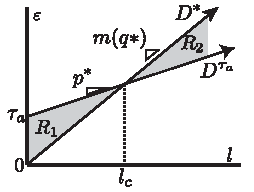
\includegraphics[width=.5\columnwidth]{img/mode-split2}
	\caption{Inefficiency of population division with access toll}
	\label{fig:mode-split}
\end{figure}

\subsection{Uniform $\ve$ or $l$}

Relaxing Assumption \ref{ass:density} permits degenerate cases of $f(\ve,l)$ for which the access toll actually \emph{can} decentralize the SO. For instance, if all travelers have the same trip length $\bar{l}$, then the population will lie along a vertical line in Fig. \ref{fig:mode-split}. Then it is efficient for traffic to be split such that only travelers with $\ve_i>\bar{l}c(q^*)$ drive, whereupon $\tau_a=\bar{l}c(q^*)$ (equal to every traveler's externality) enforces the SO. 

Alternatively, consider the case where $\ve_i=\bar{\ve}$ for every traveler; all travelers lie along a horizontal line in Fig. \ref{fig:mode-split}. In this case, only those travelers with trips shorter than $\bar{\ve}/m(q^*)$ should drive. A toll $\taua = \bar{\ve} c(q^*)/m(q^*)$ (equal to the externality of the longest trip in the SO) would split the line $\ve=\bar{\ve}$ at the correct trip length, deterring any longer trips and no shorter trips. This result resembles that obtained in \citet{Fosgerau2015}'s ``outside option'' extension (Sec. 3.2), wherein all travelers can obtain some universal reservation utility by not driving. In that model, a fixed toll deters the longest trips and achieves the SO, because ``it is the drivers with the longest trips who are at the margin'' (i.e., who obtain the least utility by driving) (p. 247). When $\ve$ varies, however, the situation is just as though some travelers' outside options were lower than others; such travelers are not as easily deterred by the fixed toll, and if their trips are especially long they greatly value the speed gains that accompany a higher toll.

\section{Aggregates}\label{sec:aggregates}

In the numerical simulations below it will be necessary to calculate aggregates for TSS (total social surplus), TCS (total consumer surplus), TR (total revenue) and $\bar{l}$ (average trip length).  To do so, we introduce a new function
\begin{equation}
	X(p,l,\taud,\taua) = (p+\taud)l + \taua
\end{equation}
that gives the disutility of a car trip of length $l$, given pace $p$ and tolls $\taua$ and $\taud$. (Depending on the tolling regime, either $\taua=0$  or $\taud=0$, since we do not consider a mixed regime, although the expressions are easily applied to one.) Thus, a traveler $i$'s private surplus is $\varepsilon_i-X(p,l_i,\taua,\taud)$. Since non-drivers receive utility 0, to calculate TCS we sum over all travelers who attain positive utility from driving:
\begin{equation}\label{eq:TCS}
	TCS = \lambda \int_{l=0}^{l=\infty} \int_{\ve=X(p,l,\taud,\taua)}^{\ve=\infty} f(\ve, l)(\varepsilon-X(p,l,\taud,\taua)) d\ve dl.
\end{equation}
The units of surplus here are veh-min/lane-km/min, so this is not a stock measure of welfare given for the total network but rather a flow measure given per lane-km of network. In the flow congestion graphical framework, this sum is equal to the area of the shaded region in Fig. \ref{fig:surplus}: the area between $p_d(q)$ and the vertical axis above the equilibrium pace $p$. The proof of this equivalence is in the appendix.

\begin{figure}
	\centering
	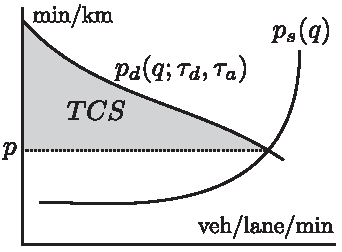
\includegraphics[width=.45\textwidth]{img/surplus}
	\caption{total consumer surplus in the flow congestion framework}
	\label{fig:surplus}
\end{figure}

Moving on, since $i$'s revenue paid is $l_i \taud + \taua$, total revenue is
\begin{equation}
	TR = \lambda \int_{l=0}^{l=\infty} \int_{\ve=X(p,l,\taud,\taua)}^{\ve=\infty} f(\ve, l)(l\taud + \taua) d\ve dl.
\end{equation}
Adding TCS and TR gives TSS, which considers only delay, as revenues are counted the same way in the toll authority's hands as in the drivers':
\begin{equation}
	TSS = \lambda \int_{l=0}^{l=\infty} \int_{\ve=X(p,l,\taud,\taua)}^{\ve=\infty} f(\ve, l)( \ve - lp) d\ve dl.
\end{equation}
Finally, the average realized trip length, $\bar{l}$, can be found by the ratio
\begin{equation}
	\bar{l} = \frac{q}{a},
\end{equation}
where $a$ is the toll-conditional arrival flow
\begin{equation}
    a = \lambda \int_{l=0}^{l=\infty} \int_{\ve=X(p,l,\taud,\taua)}^{\ve=\infty} f(\ve,l)d\ve dl
\end{equation}

\section{Numerical simulation}
\label{sec:numerical_simulation}

This section will apply the model in simulations. The purpose of simulation is to confirm that the model is computable and to demonstrate the existence and magnitudes of some of the effects about above. Section \ref{ssec:simulation_setup} explains the functional forms and parameter values chosen, while  Sec. \ref{ssec:results} presents results for several parameter combinations.

\subsection{Functional forms}
\label{ssec:simulation_setup}

To build the simulation, there are two functional forms to choose: the MFD and the population distribution $f$. The MFD is in the family given by \citet{Drake1967a} for freeway traffic: 
\begin{equation}
	p(k) = p_f \exp(-\nicefrac{1}{2}(\nicefrac{k}{k_0})^{2}),
\end{equation}
so that $q(k)$ reaches a maximum $q_0=k_0/(p_f\sqrt{e})$ at $k=k_0$. This function was chosen for its tractability. While \citet{Daganzo2012} fit a more complex model to data from Yokohama, \citet{Olszewski1995} and \citet{Williams1987a} show the exponential to fit other network data well.

The population distribution $f(\ve,l)$ is bivariate lognormal with means $(\mu_\ve, \mu_l)$ and covariance matrix 
$$
\Sigma := \begin{pmatrix}
	\sigma^2_\ve & \sigma^2_{\ve,l} \\
	\sigma^2_{\ve,l} & \sigma^2_l
\end{pmatrix},
$$
where $\sigma^2_\ve$ gives the variance of gross benefit, $\sigma^2_l$ the variance of trip length and $\sigma^2_{\ve,l}$ the covariance of gross benefit and trip length.

\subsection{Results}
\label{ssec:results}

A computer program was used to numerically calculate (i) the untolled UE; (ii) the equilibrium with TSS-maximizing access tolls; and (iii) the social optimum along with the distance toll that decentralizes it.\footnote{The code for the simulation is written in the open-source \emph{Julia} language. It is documented with instructions on how to create the table and plots and can be found at \emph{https://github.com/lewis500/distribution-of-trip-lengths}.} For safety, the optimal distance toll was calculated both numerically and via the marginal external cost rule; both methods produced the same optimal toll.

The MFD parameters were chosen to resemble the famous Yokohama experiment that produced the original MFD result in \citet{Geroliminis2008}: $k_0 = 55$ veh/lane-km and $p_f=2.2$ min/km (27.7 km/hr).

\begin{figure}
	% \centering
	\hspace*{-.1\textwidth}
	\subfloat[1][equilibria in flow congestion framework]{
	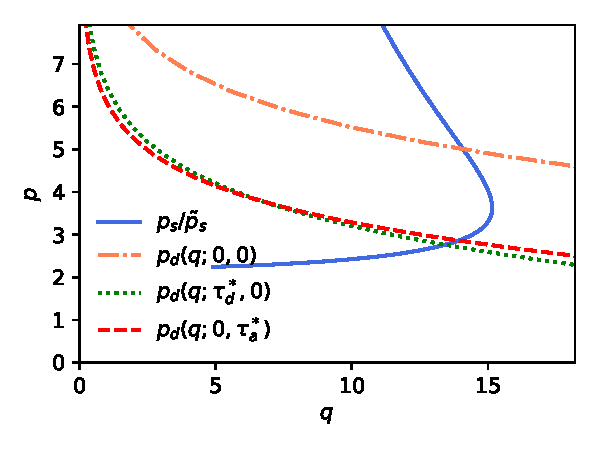
\includegraphics[width=0.55\textwidth]{img/supplyDemand}\label{fig:supplyDemand}
	}
	\subfloat[2][trip length distributions]{
	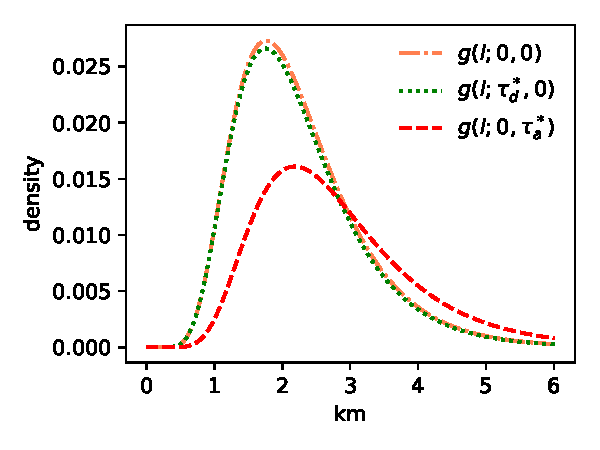
\includegraphics[width=0.55\textwidth]{img/tripLengths}\label{fig:tripLengths}
	}\\
	\hspace*{-.1\textwidth}
	\subfloat[4][division of the traveler population]{
	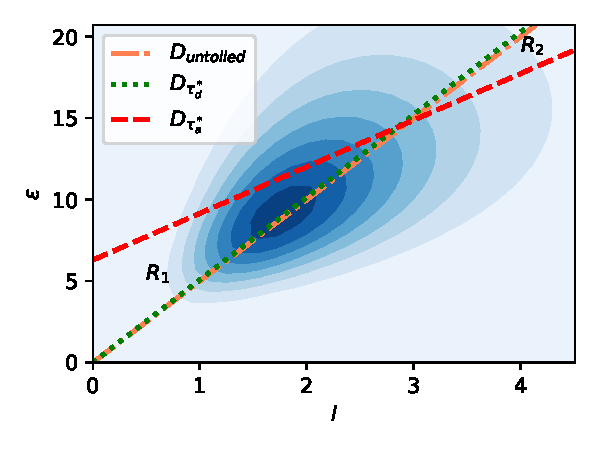
\includegraphics[width=0.55\textwidth]{img/division}\label{fig:contour}
	}
	\subfloat[4][welfare advantage of distance over access toll]{
	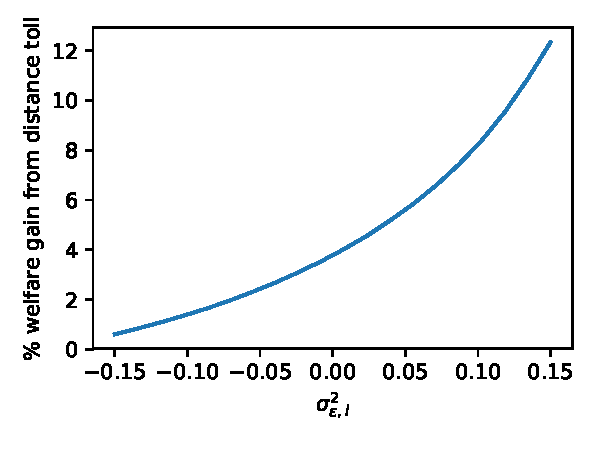
\includegraphics[width=0.55\textwidth]{img/advantage}\label{fig:advantage}
	}

	\caption{simulation results}
	\label{fig:results}
\end{figure}

First, we investigate the model under demand parameters chosen so the untolled UE exhibits moderate hypercongestion and the average trip length, 2.3 km, observed in Yokohama: $\lambda=20$, $\mu_\ve=2.4$, $\mu_l=1.0$,  $\sigma_\ve^2=\sigma_l^2=0.2$, $\sigma_{ve,l}^2=0.12$. The population's mean trip length is thus 3 km, and the mean $\ve$ is 12.2 min. For these parameters, Fig. \ref{fig:supplyDemand} shows the curves $p_s/\tilde{p}_s$ and alongside the inverse demand curves for each toll regime---with intersetions being equilibria.

\begin{table}
\centering
\begin{tabular}{l||c|c|c|c|c|c|c|c|c}
	toll & $\tau$ & $k$ & $\bar{l}$    & $p$    & $q$     & $a$    & TCS    & TR    & TSS \\ \hline\hline
none   & 0.0 & 70.5 & 2.3 & 5.0 & 14.1 & 6.0 & 20.4 & 0.0  & 20.4 \\ \hline
distance & 2.3 & 37.1 & 2.3 & 2.8 & 13.4 & 5.8 & 19.4 & 31.0 & 50.5 \\ \hline
access   & 6.3 & 39.9 & 3.1 & 2.9 & 13.9 & 4.6 & 17.3 & 28.7 & 46.0 
\end{tabular}
\caption{TSS-maximization results}\label{tab:results}
\end{table}

Statistics for each toll regime appear in Table \ref{tab:results}. The untolled UE is moderately hypercongested, with a $k>k_0=55$. All three regimes produce a similar circulation, although the tolls are able to do so with much lower paces. The distance toll achieves the highest TSS, yielding a 148\% improvement over the untolled UE and a 10\% improvement over the best-possible access toll. For both tolls, however, consumer surplus declines somewhat, although the effect is stronger for the access toll.

Turning now to the distribution of trip lengths, Figure \ref{fig:tripLengths} shows, for each toll regime, the function
\begin{equation}
	g(l;\taud,\taua) = \int_{\ve=X(p,l,\taud,\taua)}^{\ve=\infty}f(\ve,l)d\ve
\end{equation}
giving the density of realized trips by trip length, where the $p$ in the lower integral bound is the equilibrium pace induced by the given tolls. Observe that the distribution is similar without tolls and with the distance toll, because travelers respond to a toll and to a pace change in the same way. By contrast, the access toll substantially changes the distribution: the mass of trips longer than about 3km actually rises with the access toll. Consequently, the access toll causes $\bar{l}$ to rise 35\%, whereas the distance toll maintains approximately the same $\bar{l}$ as in the untolled UE. Note that, since any change in the density for a given trip length is caused by a change of equal sign in the utility for that trip, Fig. \ref{fig:tripLengths} also indicates who wins and loses from each toll change. Moreover, due to the higher $\bar{l}$, the arrival flow $a$ is much lower with the access toll even though circulation is slightly higher. Hence, an analyst focused on changes in arrival flows might rate the access toll chosen as being even more potent than the distance toll, although it reduces pace and raises welfare by a smaller amount.

Figure \ref{fig:contour} shows the population division between drivers and not-drivers under each regime, as per Fig. \ref{fig:mode-split}; travelers to the left of each $D$ line drive, and shading denotes the population density as in Fig. \ref{fig:density}. $D_{\taud^*}$ and $D_{untolled}$ are almost identical, whereas $D_{\taua^*}$ has the shallower slope and higher intercept expected. Clearly, a substantial number of trips fall into the $R_1$ and $R_2$ regions.

In this example, the access toll has been handicapped by the positive correlation between $\ve$ and $l$, which puts more mass in $R_2$ and $R_2$. As a final experiment, we change the covariance parameter $\sigma_{\ve,l}^2$ while keeping the other demand parameters constant and plot the welfare improvement gained by switching from the best-possible access toll to the best-possible distance toll. Results are plotted in Fig. \ref{fig:advantage} over the range $-.15$ to $.15$. When trip length and gross benefit are very negatively correlated, the distance toll's advantage is minor; when the two are very positively correlated, the advantage is substantial.

\section{Conclusion}
\label{sec:conclusion}

This paper has presented a static model of traffic into a downtown with an MFD, in which commuters with varying trip lengths and benefits from driving decide between driving and a zero-utility outside option. An application of Little's Law allows the user equilibrium to be derived from curves in pace/circulation space. Theory shows that an access toll cannot raise total social surplus as much as a distance toll (except in the special cases where demand is deterministic or trip lengths invariant), because it allows and even invites some long, low-value car trips while discouraging certain short, high-value car trips. The distance toll, by contrast, is able to decentralize the social optimum.


It is easy to imagine promising extensions to the model. One would involve letting the value of time vary among travelers---either in addition to or instead of having the gross benefit varying.  \citet{Meng2012} solve for optimal distance tolls in a network model where the value of time varies continuously over the population, but the model is too complex to derive rules-of-thumb and qualitative results like those of interest here. More similar is \citet{Mayet2000}. That study considers commuters with different values of time choosing whether to traverse a congestible highway, with an uncongestible road playing the role of ``outside option.'' Extending parts of that analysis to an MFD setting like ours could yield new insights, but the author's opinion is that variable value of time would not undermine the main results of this study. After all, it will remain true that long trips derive more benefit from a speed improvement than short trips, opening the door to the same inefficiencies of an access toll.

Another extension could involve time-varying conditions. It seems there are two main ways to do so. One approach, for example \citet{Gonzales2015}, is to say that trip opportunities are generated over a finite interval according to a fixed distribution of the traveler's schedules---e.g., their work start or end times. In such a model, travelers cannot reschedule their trips, but traffic conditions can change over time; the zone might fill up with cars during the beginning of the rush and empty out at the end. The author has already built a numerical, agent-based simulation to study this model; it seems that, in the middle of the rush, a steady state prevails which is exactly equivalent to the static model. 

A more realistic but more challenging approach to dynamic modelling would endow travelers with schedule preferences and give them the chance to reschedule their trips. Such a model is extremely complex, but \citet{Lamotte2017} show that, even though the untolled equilibrium in such a model cannot generally be derived analytically, some of its properties can be (a claim confirmed by the authors' simulations). A chief question for that setting is whether the tolls themselves vary dynamically and if so how to calculate the optimal tolls given the intractability of calculating the equilibrium. There is, moreover, the problem of comprehensibility: while Singapore, Stockholm and Gothenburg have all managed to implement stepwise access tolls, a dynamic distance toll might strain drivers' decision-making abilities.

Regarding policy recommendations, a tempting conclusion is that cities should switch from access to distance tolls. Distance tolls raise social welfare more than access tolls, and they allow more trips to be made, by tolling off long trips that create significant congestion---likely a political advantage. However, some caution is in order. In the first place, whereas access tolls can rely on the proven number-plate recognition and RFID technologies already used widely for bridge and highway tolls, administering a distance toll might pose challenges that are hard to foresee until such schemes have been tried. Simple as they are, even access tolls have proven at times much more expensive to set up and administer than originally planned; see the London experience \citep{santos2008}. 

More broadly, while time and experience may assuage the technical problems of distance tolling, it may be inevitable that distance tolls must by their nature invite delicate privacy concerns; such tolls requring tracking not only the vehicle's entry to or exit from a zone---as with an access toll---but the overall motion of the vehicle, too. As in the domains of security and taxation, how to balance the gains of rational policy against the dangers of a prying Leviathan will remain a puzzle for some time. One idea is that, rather than collecting information on vehicle's travel, the toll infrastructure can signal prices to devices installed on the vehicles, which then charge a stored-value card and only return a confirmation to the infrastructure. Such a scheme design, which only tracks the vehicle in the event of error, appears to be on the table for Singapore's ERP 2.0 distance-tolling system \citep{Tan2016}.

\subsection*{Acknowledgements}

The author is indebted to Carlos Daganzo, Richard Arnott, Mogens Fosgerau and two anonymous reviewers for comments that have greatly improved the paper.

\appendix

\section{Total consumer surplus}

Here we will prove that, as in \citet{Walters1961}, total consumer surplus can be calculated graphically as the area of the shaded region in Fig. \ref{fig:surplus}. To start, note that such area equals
\begin{equation}\label{eq:int-qd}
   \int_{\hat{p}=p}^{\hat{p}=\infty} q_d(\hat p,\taud,\taua)d\hat{p},
\end{equation}
so the goal is to prove that (\ref{eq:int-qd}) is equivalent to (\ref{eq:TCS}), which we will rewrite here for convenience:
\begin{equation}\label{eq:TCS2}
    TCS = \lambda \int_{l=0}^{l=\infty} \int_{\ve=X(p,l,\taud,\taua)}^{\ve=\infty} f(\ve, l)(\varepsilon-X(p,l,\taud,\taua)) d\ve\, dl.
\end{equation}

To prove the equivalence, note the integrand in (\ref{eq:TCS2}) can be transformed into an integral over benefit like so:
\begin{equation}
    f(\ve,l)\cdot(\ve - X(p,l,\taud,\taua))= \int_{x=X(p,l,\taud,\taua)}^{x=\ve} f(\ve,l) dx
\end{equation}
Replacing the integrand with this expression yields
\begin{equation}
	TCS = \lambda \int_{l=0}^{l=\infty}  \int_{\ve=X(p,l,\taud,\taua)}^{\ve=\infty} \int_{x=X(p,l,\taud,\taua)}^{x=\ve} f(\ve,l)dx\,d\ve\,  dl.
\end{equation}
Now swap the two inner integrals, changing their limits appropriately, to obtain
\begin{equation}
	TCS = \lambda \int_{l=0}^{l=\infty} \int_{x=X(p,l,\taud,\taua)}^{x=\infty} \int_{\ve=x}^{\ve=\infty} f(\ve,l)d\ve \, dx \, dl.
\end{equation}
Since $\partial X / \partial p=l$, we can apply integration by substitution---changing $x$ to a pace variable $\hat{p}$: 

\begin{equation}
	TCS = \lambda \int_{l=0}^{l=\infty} \int_{\hat p = p}^{\hat p=\infty} \int_{\ve=X(\hat p,l,\taud,\taua)}^{\ve=\infty} l f(\ve,l)d\ve \, d\hat{p}\, dl.
\end{equation}
Finally, swapping the outer two integrals and taking $\lambda$ inside yields
\begin{equation}
	TCS = \int_{\hat{p}=p}^{\hat{p}=\infty} \left( \lambda \int_{l=0}^{l=\infty} 
		\int_{\ve=X(s,l,\taud,\taua)}^{\ve=\infty} lf(\ve,l)d\ve
	dl \right) ds,
\end{equation}
where the term in $(\cdot)$ is equal to $q_d(p,\taud,\taua)$, as required.


\pagebreak
\subsection*{References}
\bibliographystyle{elsarticle-harv}
\bibliography{distance,practice}

\end{document}